\chapter{Deep autotuner: technical presentation of the proposed system}
\label{chap:thesis-autotuner}
In this chapter, I describe the proposed autotuning system, which I call \textit{Deep Autotuner} \cite{wager2020deep}. I start by discussing related work in pitch correction. Given that not much work has been done on the topic, I consider work on similar tasks such pitch detection, and relevant techniques in the larger areas of deep learning and signal processing. I then describe in detail the structure of the neural network, the data preparation steps---including de-tuning and feature extraction, the training configuration, and the experimental setup. 

%Introduction
%- based on chapters 2 and 3 (ok)
%- empirical (ok)
%- data-driven (ok)
%- applies to any culture it is trained on
%- overview

The autotuning system introduced in this thesis is a data-driven approach to automatic pitch correction of solo singing performances. The proposed approach predicts note-wise pitch shifts from the relationship between the respective spectrograms of the singing and accompaniment. It outputs the amount and direction of the pitch shift expected to bring the note back in tune, without requiring access to the musical score. This makes it usable even when the singer improvises or harmonizes in a performance.

Automatic pitch correction---``autotuning"---is difficult. For example, a notated musical score is a sequence of notes of discretized lengths and pre-defined pitches. The simplicity of the symbolic representation leaves considerable scope for variation in the singer's interpretation. Hence, although a vocalist follows the general contour of the score, and the result sounds in tune, the singing voice actually varies continuously due to expressive gestures such as pitch bending, vibrato, and any other variations coming from the different genres and personal styles. The proposed data-driven approach tries to respect the nuanced variations of sung pitch, while the system also actively estimates the amount of unintended pitch shift (see Fig. \ref{fig:results}).

\begin{figure}[t]
    \centering
    \includegraphics[width=\columnwidth]{figures/results.pdf}
    \caption{An example of the behavior of the proposed autotuner model. The red line shows the pitch contour of the vocal track input to the model. The green line shows the pitch contour after applying corrections predicted by the Deep autotuner. This plot shows a synthesized training example: The black line shows the original vocal track pitch contour, which was de-tuned to the red line to generate an input-target pair for supervised training.}
    \label{fig:results}
\end{figure}

The proposed system is designed to utilize similar information as the human ear, basing corrections on information found in the audio, such as the level of perceived musical harmony and context in time. It is a neural network trained on patterns in real-world singing examples. This approach differs from commercial systems such as Antares Auto-Tune, where vocal track notes are usually shifted to be centered around pitches in a user-defined score, or mapped to the closest pitch among the twelve equal-tempered scale degrees. The proposed system treats pitch as a continuous value rather than relying on a set of discretized notes found in musical scores. The design of the proposed system is based on the empirically derived conceptualization of musical intonation described in Section \ref{sec:empirical}. It is a step towards a model-free autotuning system, the use of which I justify in Chapter \ref{chap:tech-background}. 

I train the neural network model using a dataset of 4,702 amateur karaoke performances selected for good intonation. The model is trained on both incorrect intonation, for which it learns a correction, and intentional pitch variation, which it learns to preserve. The proposed deep neural network with gated recurrent units on top of convolutional layers shows promising performance on the real-world score-free singing pitch correction task. To the best of my knowledge, the proposed method is the first data-driven approach to correcting singing voice pitch based on its harmonic alignment to the accompaniment.

\section{Open-source repository}
%- code is available
An implementation of the system Python and Pytorch is available to the public at \href{https://github.com/sannawag/autotuner}{https://github.com/sannawag/autotuner}. Users have the option of training the model on their own dataset or of downloading the parameters of the model that provided the best test results. The repository also includes code for a baseline autotuning system introduced in \ref{sec:subjective-test}, and an implementation of the time-domain pitch-synchronous overlap and add (TD-PSOLA) algorithm \cite{charpentier1986diphone}.

\section{Related work}
%related work
%pitch correction
%- mention antares
The first commercial pitch-correction technique, Antares Auto-Tune \cite{antares:2016}, is also one of the most commonly used. Section \ref{sec:autotune} describes in detail how it works. Auto-Tune measures the fundamental frequency of the input monophonic singing recording, then re-synthesizes the pitch-corrected audio signal. In Auto-Tune and in recent work on continuous score-coded pitch correction \cite{salazar2015continuous}, each vocal note is pitch shifted to the nearest note in a user-input set of pitches (scale) or to the pitch in the score if it is known. The default musical scale is the equal-tempered scale, in which each pitch $p$ belongs to the set of MIDI pitches $[0, 1, ..., 127]$ and its frequency in Hertz is defined as $440*2^{\frac{p-69}{12}}$. Some users prefer a finer resolution and include more than twelve pitches per octave, or use intervals of varying sizes between pitches. In any case, the fundamental frequency is discretized to a small set of values, around which every note is shifted to be exactly centered. Hence, the pitch shifts tends to ignore a singer's intentional expressive gestures and might not easily apply to non-Western music with different scales or more fluidly varying pitch. The proposed system accommodates this variety of frequencies by letting the fundamental frequency take any value along a continuous scale, and by shifting every note by a constant without modifying internal pitch variation.

%- other pitch correction programs
Recent style-transfer-based work modifies amateur performances to mimic a professional-level performance of the same song. Luo \textit{et al.} proposed to match the pitch contour of the professional-level performance while preserving the spectral envelope of the amateur performance \cite{luo2018singing}. Meanwhile, Yong and Nam proposed to match both the pitch and amplitude envelopes \cite{yong2018singing}. Our model is similar in the sense that it also uses features gathered from high-quality performances \cite{wager2018intonation}. However, the proposed model does not necessitate a ``target" performance of the same song during testing. Instead, it learns from many in-tune singing voice examples and their accompaniments, and then generalizes to unknown songs, while preserving the original singer's style.

\subsection{Music information retrieval}
%pitch detection
%    - pitch detection
%    - CQT
%    - WaveNet?
Music Information Retrieval (MIR) research on related tasks such as pitch detection provides a useful background for this thesis. Gomez {\it et al.}\cite{gomez2018deep} provide an overview of recent developments in deep learning for singing processing, ranging from pitch detection to singing separation and synthesis. We focus here on pitch detection as it is particularly relevant to autotuning. It also aims to extract harmonic patterns from the audio, which correspond to perceived pitch. In the case of pitch detection, the perceived pitches are often manually annotated. 

Bittner \textit{et al.} introduce a fully convolutional DNN for polyphonic pitch transcription. The input is the magnitude harmonic constant-Q transform of the audio. The constant-Q transform (CQT) is a time-frequency transformation suitable for a convolutional neural network. It can be contrasted to the Fourier transform, which has linearly spaced center frequencies $f_n = n * \frac{SR}{N}$, where $n$ is the frequency bin index, $SR$ is the sampling rate, and $N$ is the dimension of the transformation space. The CQT instead has logarithmically spaced center frequencies $f_j = f_{min} * 2^{\frac{j}{b}}$ where $f_{min}$ is a pre-defined minimum frequency and $b$ determines the number of bins per octave. The fact that the center frequencies are logarithmically spaced results in the audio representation being translationally invariant, meaning that shifting a musical interval up or down will not change its spacing in the CQT. This enables a CNN filter to discover harmonic patterns across the full range of frequencies. Another advantage of the CQT representation is that it has a similar resolution to the human auditory system, with high resolution in the lower frequencies and wider bins in the higher frequencies. The downside of using CQT is that it cannot benefit from the Fast Fourier transform optimization, so is computationally expensive, $\mathcal{O}(N^2)$ instead of $\mathcal{O}(N \log (N))$. Bittner \textit{et al.} add more resolution by computing multiple, overlapping CQTs, each starting at a different frequency. This technique is called harmonic CQT (HCQT). The network structure includes four lower layers with small filters of dimension $5 \times 5$ or $3 \times 3$ to detect small-scale patterns. The fifth layer, instead, uses a filter that spans an octave of audio. This musically informed network design decision increases the relevant receptive field of each output state---the context in the input HCQT it can access---without needing to make the network very deep. The sixth layer then uses a $1 \times 1$ filter to combine all the learned features and output a pitch activation map. \cite{bittner2017deep} The DNN proposed in this thesis utilizes CNN layers whose structure is closely based on this network. Since our pitch correction task is sensitive even to a small amount of pitch shift, we also choose to use the CQT for its finer resolution in the lower frequencies. 

Basaran {\it et al.} add to the pitch detection CNN by adding a recurrent layer to incorporate the sequential nature of audio and music signals into their DNN structure. The network estimates the main melody in polyphonic audio signals in the constant-Q transform (CQT) representation, using a gated recurrent unit (GRU) layer \cite{chung2014empirical, ChoK2014arxiv} to model the temporal structures \cite{basaranmain}. 

\subsection{Deep learning}
%deep learning and audio
%- related deep learning
%    - singing processing

%    - Amazon paper for CNN + rnn structure + pre-training
\subsection{Audio signal processing}
%pitch shifting
%- PSOLA: TD-PSOLA algorithm \cite{charpentier1986diphone}
In future work, we plan to explore other pitch processing techniques in training, such as \cite{waloschek2018driftin}.
% probabilistic YIN --> also inspires own approach to HMM note parsing

\begin{figure*}[t]
\subfigure[]{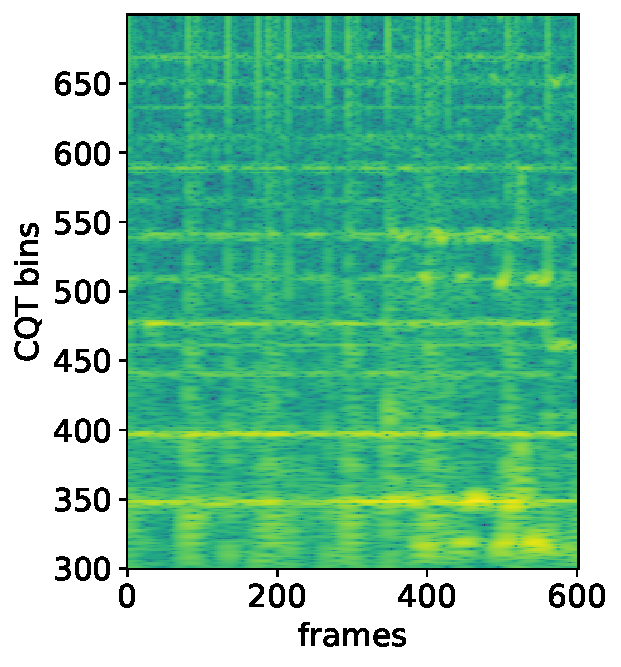
\includegraphics[height=1.625in]{figures/cqt_comparison_1.pdf}}\hspace{-.15in}%\vspace{-.03in}
\subfigure[]{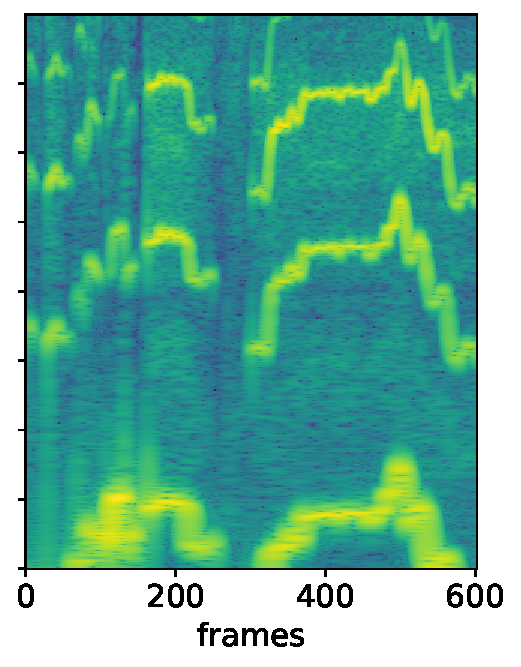
\includegraphics[height=1.625in]{figures/cqt_comparison_2.pdf}}\hspace{-.15in}%\vspace{-.03in}
\subfigure[]{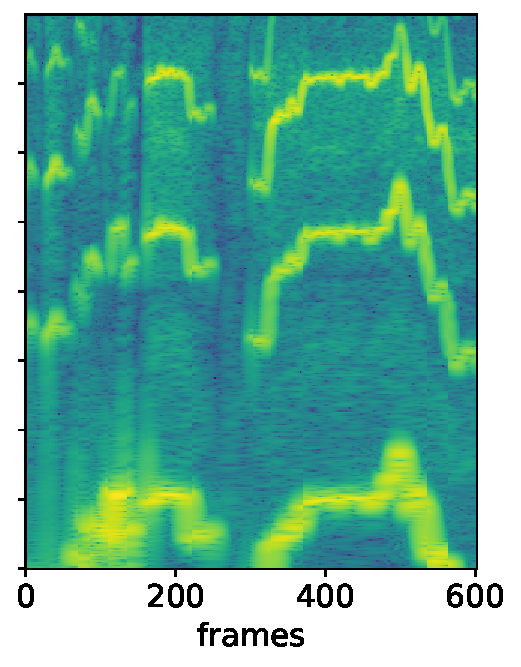
\includegraphics[height=1.625in]{figures/cqt_comparison_3.pdf}}\hspace{-.15in}%\vspace{-.03in}
\subfigure[]{\includegraphics[height=1.625in]{figures/cqt_comparison_4-2.pdf}}\hspace{-.15in}%\vspace{-.03in}
\subfigure[]{\includegraphics[height=1.625in]{figures/cqt_comparison_5-2.pdf}}\hspace{-.15in}%\vspace{-.03in}
    \caption{
    Constant-Q transform of the vocals and backing tracks using \cite{mcfee2015librosa}. We zoom into bins 300 through 700 for better visibility. (a) shows the CQT of the backing track. The horizontal lines are due to constant pitches. (b) and (c) show the CQT of the vocals before and after the correction, respectively. (d) and (e) show the binarized CQT of the superposed vocals and backing track before and after corrections (see Section \ref{sec:data-format-autotune}). The correction shifted the pitch of the vocals up and centered it around the desired harmonics of the backing track (red circles). 
    }
    \label{fig:model-input-autotune}
\end{figure*}

%Proposed model
\section{The proposed pitch correction system}
\label{sec:proposed-autotune}
 
%- harmonic alignment (see the proposed pitch system)
Our proposed model predicts pitch correction based on the harmonic alignment between the vocals and backing tracks. We assume that the backing track has clearly identifiable pitches---a chord progression---which serves as a reference for the vocals.

The accompaniment track remains fixed.  
%    - applies to any culture it is trained on
%- time-frequency representation overview
%    - CQT
A time-frequency representation is a natural approach for extracting information about the harmonics across a sequence of notes. Fig. \ref{fig:model-input-autotune} shows the CQT of vocals and backing track clips before and after applying predicted pitch corrections. It also shows how these shifts affect the harmonic structure of the two tracks combined. Given such data, the proposed model uses convolutional neural network (CNN) layers followed by a GRU to extract sequential patterns of harmonic alignment. It predicts pitch shifts that will align the vocals with the backing track. 
%- supervised training pairs. discuss this in data sec.
Training data consists of pairs of performances that are identical except for the vocals pitch. Such pairs, while required to train the model, are difficult to come across naturally. Hence, we synthesize them by detuning high-quality singing performances to construct the input signals, and then train our model to predict the shifts that recover the original pitches (The accompaniment track remains fixed).  
%- note splitting
%    - Discretization for control, constant shift
We make the strong assumption that a singer targets a specific frequency per note, around which all pitch variations are centered. Given this assumption, we correct the pitch of one note by shifting all frames that belong to that note by a constant.

The first step in detuning is to find the note boundaries from the original singing performance as our program does not utilize a musical score. We define every transition silence as a note boundary. To this end, we analyze the vocals pitch using the frame-wise probabilistic YIN (pYIN) algorithm \cite{mauch2014pyin}, implemented as a Vamp plugin in \cite{cannam2010sonic}. We then shift every note by a random amount along the continuous logarithmic scale of cents. We generate 7 detuned versions of each song. While our note parsing technique fails to split notes when they are connected, we assume this is not a big problem during training, because the ground truth notes are all assumed to be in-tune. This means that when they are detuned together, the same shift will apply to both. In testing, we used a different technique to compute note boundaries, as described in Section \ref{sec:experiments-autotune}.
%    - hmm for note splitting
%        - now set up for equal-tempered for simplicity
%        - could set up a fine-grained scale, 22 notes as %in raga, or any other customization
% could, in the future, try WaveNet
%- model structure with CNN and RNN
\subsection{Neural network structure}
Our model consists of stacked convolutional layers followed by a GRU layer. The last output of the GRU is fed to a dense layer that predicts a single scalar output, the note-level pitch shift. The convolutional filters pre-process the spectrogram tensor, reducing its dimensionality while also learning abstract features. Next, we keep the last output of the GRU to reduce the representation of a variable-length note to a fixed-length vector.

We use the GRU recurrent structure as a way for the model to analyze the singer's note contour, which can last a second or multiple seconds, while smoothing over unpitched or noisy sections. This is crucial because the algorithm is expected to rely on aligning harmonics, which only occur in pitched sounds. Another advantage of using the GRU is that we can use the hidden state output by one note to initialize the hidden state for the following note. Even when using our simple detuning model that shifts every pitch by an independent amount, we assume that some information from past notes (e.g. from the accompaniment track) is useful.

\begin{table}[t]
  \begin{center}
    \caption{The proposed network architecture.}
    \begin{tabular}{|c||c|c|c|c|}
    \hline
      & Conv1 & Conv2 & Conv3 & Conv4 \\
      \hline
      \#Filters/Units & 128 & 64 & 64 & 64 \\
      Filter size & (5, 5) & (5, 5) & (3, 3) & (3, 3) \\
      Stride & (1, 2) & (1, 2) & (2, 2) & (1, 1) \\
      Padding & (2, 2) & (2, 2) & (1, 1) & (1, 1) \\
      \hline
      & Conv5 & Conv6 & GRU & FC \\
      \hline
      \#Filters/Units & 8 & 1 & 64 & 1 \\
      Filter size & (48, 1) & (1, 1) & & \\
      Stride & (1, 1) & (1, 1) & & \\
      Padding & (24, 1) & (0, 0) & & \\
      \hline
    \end{tabular}
    \vspace{-.1in}
    \label{tab:network}
  \end{center}
\end{table}

Table \ref{tab:network} displays the structure of the proposed network. Given that the input is a spectrogram, its meaning is different along the time and frequency axes, unlike images. For this reason, instead of max pooling, we use strides of two in the time axis in three of the convolutional layers. In the third layer, we also stride along the frequency axis, but perform this only once to not lose too much frequency information. The fifth convolutional layer has a filter of size 48 in the frequency domain, which captures frequency relationships in a larger range of the CQT, as shown to be successful in \cite{bittner2017deep} and \cite{hsu2017learning}. The error function is the Mean-Squared Error (MSE) between the pitch shift estimate and ground truth over the full sequence of notes in a performance. The MSE corresponds to deviation in cents using the formula $\left|\text{cent error}\right| = 100 * \sqrt{\text{MSE}}$.

% - predict shift, apply it later
We apply predicted pitch corrections to test performances. Unlike in training, where we shifted the magnitude CQT and ignored the phase, we use the more computationally expensive TD-PSOLA algorithm \cite{charpentier1986diphone} to detune the signals in the time domain. Furthermore, we compute note boundaries using the pYIN note-level pitch analysis, which splits notes even when there is no silence, but which we consider more prone to errors than our conservative approach in training. 
%- option of adding additional song-rnn
%- post-processing focus

%Dataset
%- Intonation introduction, refer to chapter
%    - genres in the dataset
%Real-world dataset
%- real-world set for testing
\subsection{Dataset}
\label{sec:dataset-autotune}
We construct our training dataset by deriving from the ``Intonation" dataset \cite{wager2018intonation}, which we assume to be a collection of in-tune singing voice tracks. A detailed description of the dataset is available in chapter \ref{sec:thesis-damp}. The 4702 separate vocal tracks in the dataset are mostly of Western popular music, collected by Smule, Inc, a singing app, for good intonation. While these real-world recordings contain some artifacts, no particular signal processing---e.g. denoising or filtering---has been applied to them. Each recording contains one minute of a performance, starting 30 seconds into the song. Although they are assumed to be in tune, this is not always exactly the case as the users are not necessarily professional singers. Overall, the sung pitch is quite accurate compared with the intended pitch. Hence, we treat this paper as a proof of concept. The model can be trained on professional singing for best results.

Using the metadata indicating the backing track and user index, we split the dataset into 4561 training performances, 49 validation performances, and 64 test performances. The training set contains 709 backing tracks performed by 3468 different users, while the validation set is with 17 tracks sung by 43 users and the test set is with 16 sung by 62. There is no overlap in the backing tracks across the three sets. We allow for overlap in the singer ID between the training and validation sets, but not with the test set. 

We also create another real-world test set using the test backing tracks for a subjective listening test. Outside of Smule, we recorded 8 volunteers singing along with them. Singing experience ranged from beginner to semi-professional. The singers chose what to sing, and selected a total of 7 different arrangements. We recorded a total of 24 performances. Singers familiarized themselves with their chosen songs before the recording session. During the performance, they listened to the backing track through headphones so that it would not interfere with the vocals recording. 
%De-tuning process
\subsection{The detuning process}
The synthetic pitch deviations used to construct training examples are limited to one semitone (100 cents) in either direction, a larger interval than the standard score-free approach of snapping to the nearest pitch, which limits the shift to 50 cents. In practice, it prevents errors in cases where the required shift is greater than 50, but can lead to degradation of the prediction accuracy on a too badly detuned input. We make the strong assumption is that the detuning process between notes is independent.

To detune the training data, we shift the magnitude CQT up or down. This is expected to not produce too noticeable artifacts that the program could learn instead of the pitch relationships. The one issue is formant shifting, but this is not a big concern when only shifting up to $\pm$100 cents. 
%- data de-tuning, different versions
%    - runif
%    - hmm
%        - MIR-1K
%Pre-processing details
\subsection{Data pre-processing details/Format}
\label{sec:data-format-autotune}
We convert the normalized audio signals using the CQT for its translational invariance along the frequency axis. The CQT process covers 5.5 octaves with a resolution of 16 bins per semitone. The lowest frequency is 125 Hz. The top and bottom 16 bins are used as a buffer for pitch shifting, then truncated so that every input has dimension 1024. We use a frame size of 92 ms and a hop size of 11 ms. The vocals and accompaniment CQTs form two of the three input channels to the neural network. For the third channel, to contrast the difference between the first two channels, we binarize the two CQT spectrograms using the mean modulus as a threshold, a technique used in computer vision \cite{sezgin2004survey}. We then take the bitwise disagreement of the two matrices based on the assumption that the in-tune singing voice, better aligned with the accompaniment track, will cancel out more harmonic peaks than the out-of-tune tracks. Fig. \ref{fig:model-input-autotune} illustrates the data format. In future work, we plan to explore different input formats, including omitting the binarized channel.
%- CQT parameters, etc…
%- tried third channel, did not help
%- tried the binary channel but did not help (plot)?
%- Tried TD-PSOLA, expensive but not better


%Experimental setup
\section{Experimental setup}
\label{sec:experiments-autotune}
\subsection{Training setup}
We use the Adam optimizer \cite{kingma2014adam}, initialized with a learning rate of 0.00005. We feed one note at a time to the model as a minibatch of seven differently pitch-shifted versions. We apply gradient clipping \cite{pascanu2013difficulty} with a threshold of 100. We measure validation loss every 500 songs and save the model with the best result. 
%- loss function, etc…
%- Adam
\subsection{Initialization}
The convolutional parameters are initialized using He \cite{he2015delving}, and the GRU hidden state of the first note of every song is initialized using a normal distribution with $\mu=0$ and $sd=0.0001$.
%- initialization of weights
%- pre-training
%Experiments
%- runif by note
%- hmm by note
%- runif by sequence
%- hmm by sequence
%- learning rates
%- + pre-training